\documentclass[a4paper,11pt]{article}

\usepackage[polski]{babel}
\usepackage[utf8]{inputenc}
\usepackage[T1]{fontenc}
\usepackage{graphicx}
\usepackage{epstopdf}

\title{Sprawozdanie z zajec laboratoryjnych nr 2}
\author{Radosław Chudy}

\begin{document}

\maketitle

\section{Opis ćwiczenia}
W ćwiczeniu należało zaimplementować 2 struktury danych - stos oraz kolejkę. Implementacja została wykonana na kilka sposobów. Pierwszy polegał na wykonaniu stuktur w oparciu o tablice alokowana dynamicznie. Drugi zaś wykorzystywał szablon listy dostępny z kontenera STL. Ponadto po zaimplementowaniu struktur wykonać należało test wczytywania danych do nich oraz zmierzyć czas tych operacji. Wyniki oraz graficzna reprezentacja danych znajduje się w kolejnym punkcie sprawozdania.

\section{Wyniki pomiarów}
\begin{enumerate}
 \item Stos zaimplementowany przy pomocy listy:
  \begin{figure}
  \righting
  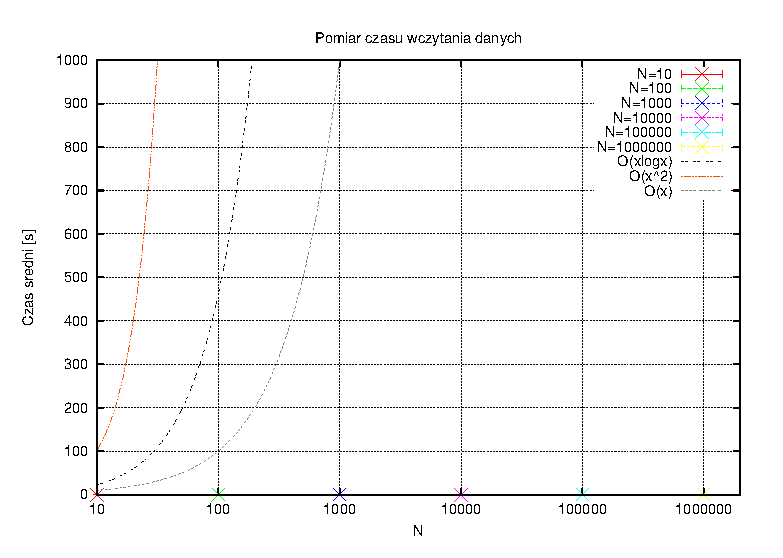
\includegraphics{wykres_dla_stoslista.eps}
  \label{Test nr 1}
 \end{figure}

 \end{enumerate}

 \section{Wnioski}
Po przeanalizowaniu uzyskanych wykresow jak i danych pomiarowych wynika iż wczytywanie danych do struktur zaimplementowanych do tablic alokowanych przez kazdoroazowe zwiekszanie rozmiaru tablicy o 1 jest mniej efektywne niż do pozostałych struktur. Złożoność obliczeniowa takiej operacji wynosi $ O(n^{2}) $ . Natomiast implementacja zarówno dla struktur na bazie listy oraz tablicy alokowanej dynamicznie przy wypelnieniu tablicy zwiekszajacej swojej rozmiar dwukrotnie jest efektywniejsza. Złożoność obliczeniowa wynosi $ O(n) $. Dzieje się tak ponieważ przy kazdorazowym wypełnieniu w stukturach listy i tablicy zwiekszanej 2 razy nie sa zwiekszane rozmiary pamieci przez co ograniczona jest ilosc operacji przepisywania elementow do struktur tymczasowych.
 \end{document}